\selectlanguage{english}%

\chapter{Implementação} \label{capImp}
Uma vez que se tenha modelado o sistema, é necessário realizar a identificação dos parâmetros da planta real afim de aplicar os mesmos passos para a sintonia do controlador. A implementação em bancada inicia-se com a calibração dos sensores e identificação dos ganhos das bombas e do sistema em 4 pontos, que irão compor os conjuntos das regras TS. Por fim, os ganhos são calculados desenvolvendo-se as matrizes de cada uma das regras e seguindo as \jhhref{eqContFuzzy}{equações}.

\section{Identificação}
Há diversas formas de realizar a identificação de um sistema. Baseando-se na forma e quantidade de informações disponíveis, existem três tipos de identificação:
\begin{itemize}
	\item \textbf{Caixa-Branca:} ocorre quando é realizada aferindo-se diretamente todos os parâmetros envolvidos.
	\item \textbf{Caixa-Preta:} baseia-se completamente nos dados externos do sistema como seus resultados para algum teste para identificação desejada.
	\item \textbf{Caixa-Cinza:} é realizada a partir de informações internas aferidas diretamente do sistema utilizando resultados externos para determinação dos parâmetros ainda não identificados.
\end{itemize}

Neste trabalho utilizou-se inicialmente o software MATLAB em uma tentativa de realizar uma identificação caixa-preta, puramente baseada nos dados obtidos a partir de degraus nas entradas. Como será visto a seguir, está abordagem não forneceu um sistema condizente com o esperado, portanto optou-se por seguir a estratégia caixa-cinza para realizar a identificação. As descrições de ambas são apresentadas a seguir.

\subsection{Identificação Caixa-Preta}
A identificação caixa-preta verifica o comportamento das saídas em relação às entradas e tenta inferir, por meio de algoritmos de regressão e outros, as equações que descrevem a dinâmica do sistema. Assim, as imagens \ref{imgID_4000} - \ref{imgID_6000} a seguir apresentam as respostas do sistema aos degraus nas entradas. Esses dados foram tratados e enviados para a Toolbox de Identificação do Matlab. 
\begin{figure}[H]
	\centering
	\begin{tabular}{cc}
		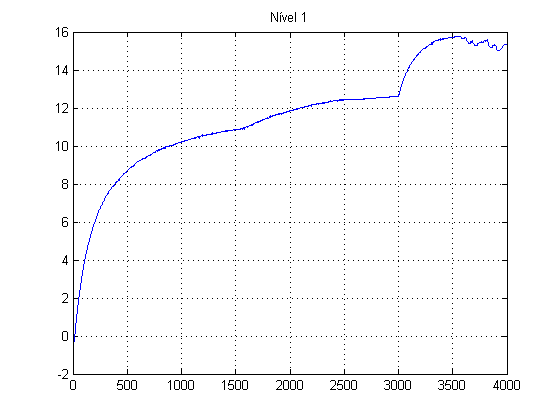
\includegraphics[height=0.15\paperheight,keepaspectratio]{img/sim1_h1.png} &
		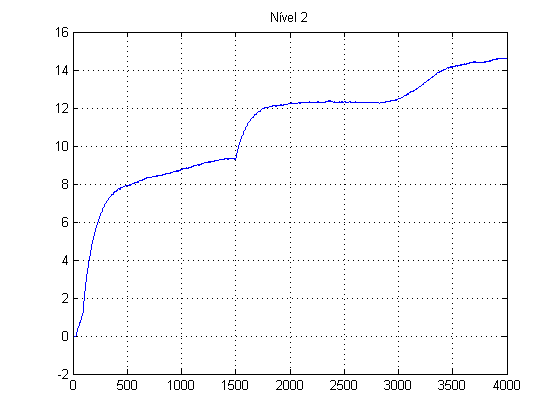
\includegraphics[height=0.15\paperheight,keepaspectratio]{img/sim1_h2.png} \\
		(a) Nível 1 &
		(b) Nível 2 \\
		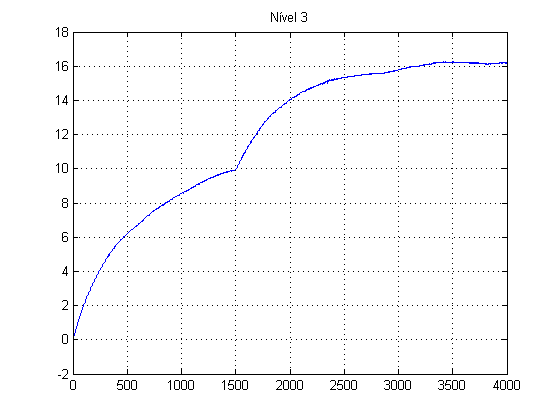
\includegraphics[height=0.15\paperheight,keepaspectratio]{img/sim1_h3.png} &
		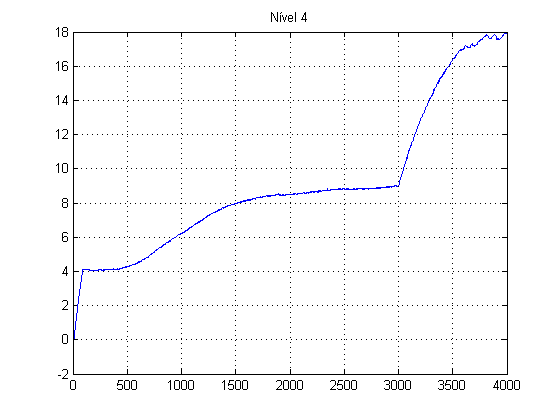
\includegraphics[height=0.15\paperheight,keepaspectratio]{img/sim1_h4.png} \\
		(c) Nível 3 &
		(d) Nível 4
	\end{tabular}
	\caption{\label{imgID_4000} Identificação 1 - 4000 segundos}
\end{figure}

\begin{figure}[H]
	\centering
	\begin{tabular}{cc}
		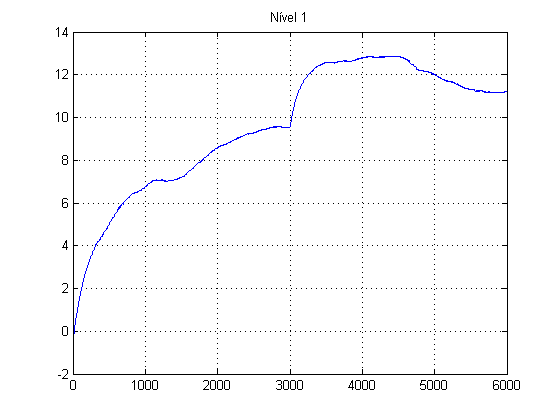
\includegraphics[height=0.15\paperheight,keepaspectratio]{img/sim2_h1.png} &
		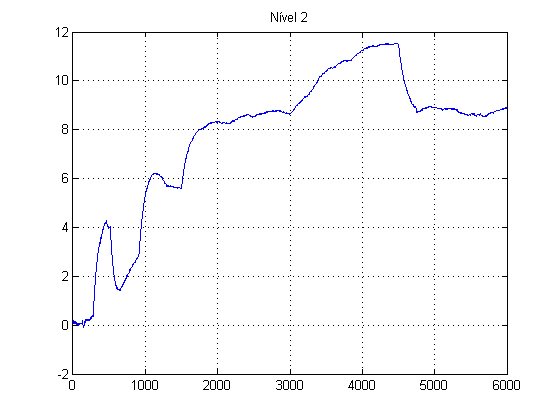
\includegraphics[height=0.15\paperheight,keepaspectratio]{img/sim2_h2.png} \\
		(a) Nível 1 &
		(b) Nível 2 \\
		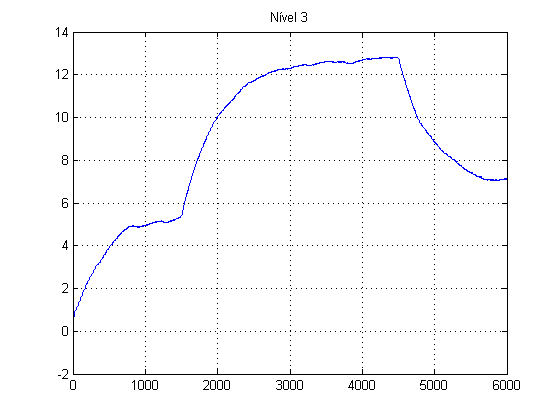
\includegraphics[height=0.15\paperheight,keepaspectratio]{img/sim2_h3.png} &
		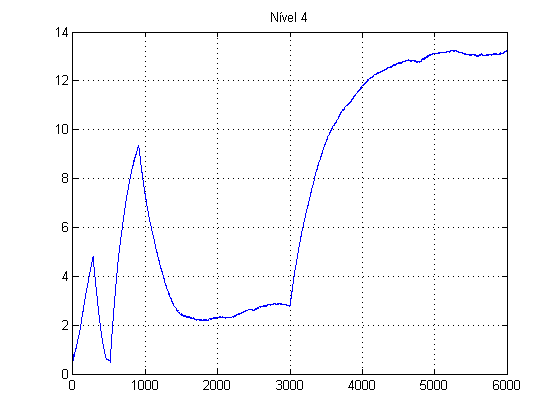
\includegraphics[height=0.15\paperheight,keepaspectratio]{img/sim2_h4.png} \\
		(c) Nível 3 &
		(d) Nível 4
	\end{tabular}
	\caption{\label{imgID_6000_v1} Identificação 2 - 6000 segundos}
\end{figure}

\begin{figure}[H]
	\centering
	\begin{tabular}{cc}
		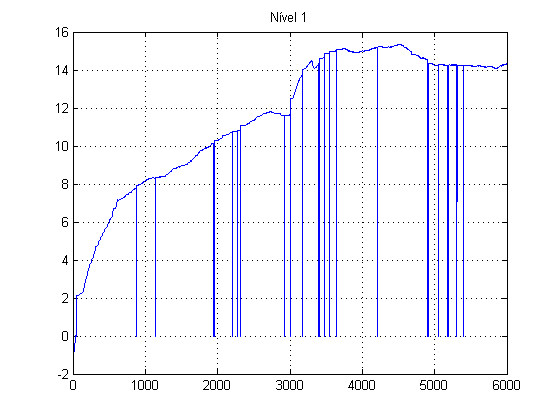
\includegraphics[height=0.15\paperheight,keepaspectratio]{img/sim3_h1.png} &
		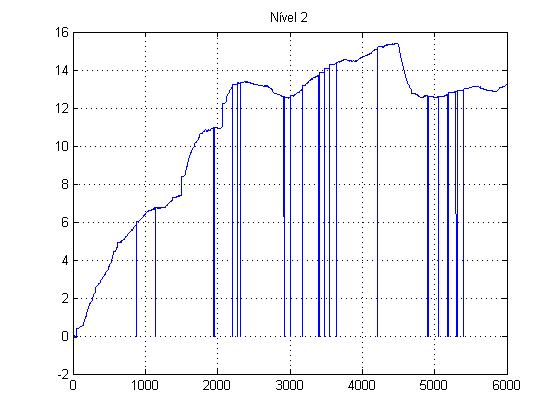
\includegraphics[height=0.15\paperheight,keepaspectratio]{img/sim3_h2.png} \\
		(a) Nível 1 &
		(b) Nível 2 \\
		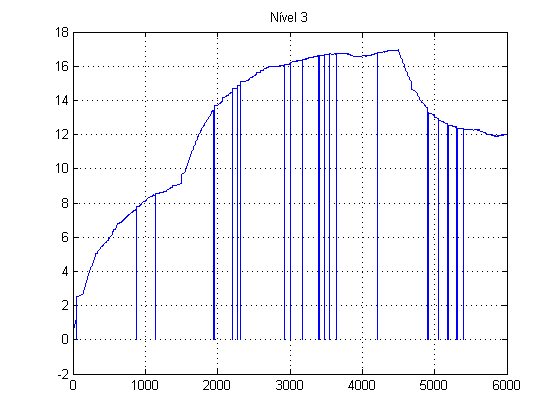
\includegraphics[height=0.15\paperheight,keepaspectratio]{img/sim3_h3.png} &
		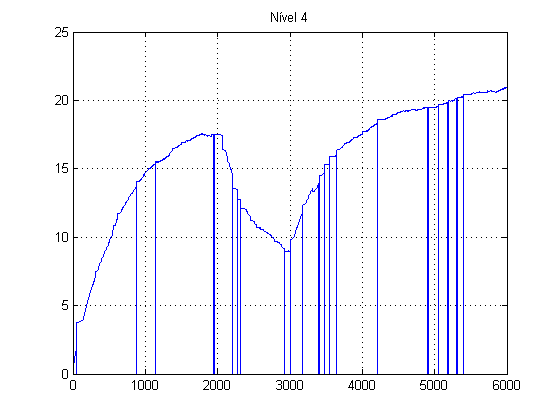
\includegraphics[height=0.15\paperheight,keepaspectratio]{img/sim3_h4.png} \\
		(c) Nível 3 &
		(d) Nível 4
	\end{tabular}
	\caption{\label{imgID_6000} Identificação 3 - 6000 segundos}
\end{figure}

A ferramenta recebe os dados de entrada e saída dos testes do sistema para estimação que retorna as matrizes índices no espaço de estados. É possível determinar as ordens dos parâmetros para estimação e quais elementos de cada matriz são conhecidos. Neste trabalho, determinou-se:

\begin{align}
	& A =
	\begin{bmatrix}
		a_{1,1} & a_{1,2} & a_{1,3} & a_{1,4} \\
		a_{2,1} & a_{2,2} & a_{2,3} & a_{2,4} \\
		a_{3,1} & a_{3,2} & a_{3,3} & a_{3,4} \\
		a_{4,1} & a_{4,2} & a_{4,3} & a_{4,4}
	\end{bmatrix}
	& B =
	\begin{bmatrix}
		b_{1,1} & b_{1,2} \\
		b_{2,1} & b_{2,2} \\
		b_{3,1} & b_{3,2} \\
		b_{4,1} & b_{4,4}
	\end{bmatrix} \\
	& C  = 
	\begin{bmatrix}
		1 & 0 & 0 & 0 \\
		0 & 1 & 0 & 0 \\
		0 & 0 & 1 & 0 \\
		0 & 0 & 0 & 1
	\end{bmatrix} 
	& D  = 
	\begin{bmatrix}
		0 & 0 \\
		0 & 0 \\
		0 & 0 \\
		0 & 0
	\end{bmatrix}
\end{align}

Os parâmetros que se deseja encontrar são $a_{i,j}$ e $b_{i,j}$. A matriz D é nula e C é a identidade, selecionando os quatro níveis, que compõe o estado, como as saídas. Os resultados obtidos são apresentados a seguir:

\begin{itemize}
\newpage \item  Identificação I:

\begin{figure}[H]
	\centering
	\begin{tabular}{cc}
		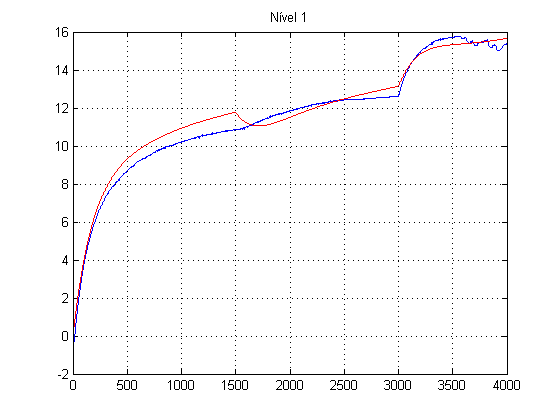
\includegraphics[height=0.15\paperheight,keepaspectratio]{img/ident1_h1.png} &
		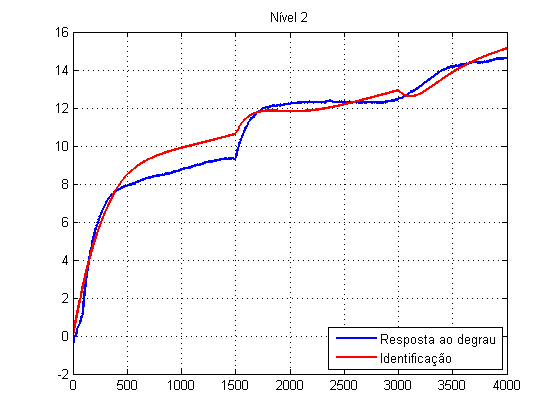
\includegraphics[height=0.15\paperheight,keepaspectratio]{img/ident1_h2.png} \\
		(a) Nível 1 &
		(b) Nível 2 \\
		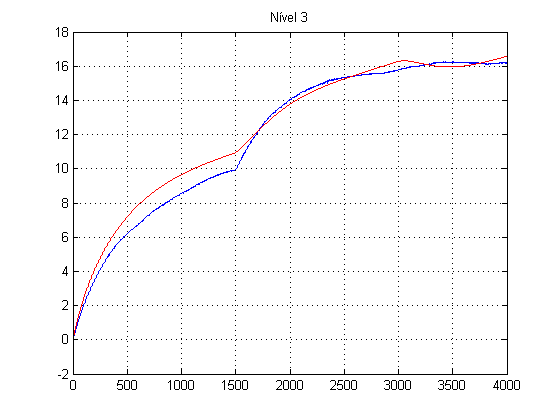
\includegraphics[height=0.15\paperheight,keepaspectratio]{img/ident1_h3.png} &
		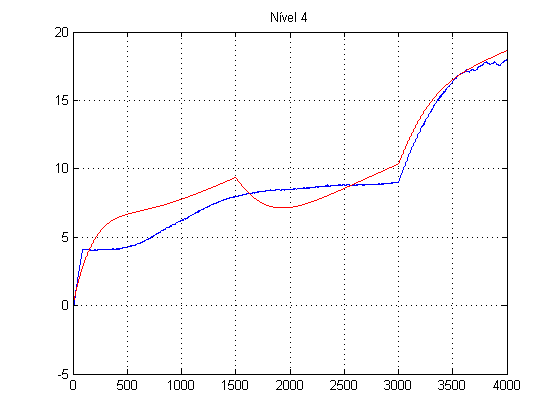
\includegraphics[height=0.15\paperheight,keepaspectratio]{img/ident1_h4.png} \\
		(c) Nível 3 &
		(d) Nível 4
	\end{tabular}
	\caption{\label{imgID_4Results} Identificação 1 - 4000 segundos}
\end{figure}

\begin{align*}
	& A_1 =
	\begin{bmatrix}
			0.9985 & -0.0002098 &  0.0007881 & 0.0001684 \\
		  0.000169 &      0.999 & -7.159e-05 & 0.0004413 \\
		 -0.000736 &  0.0001313 &          1 & 0.0001939 \\
		-0.0009293 & -0.0008117 &    0.00109 &         1
	\end{bmatrix}\\
	& B_1 =
	\begin{bmatrix}
		-0.0006189 &  0.0008599 \\
		  0.000715 & -0.0005701 \\
		 0.0001636 &  -2.26e-05 \\
		-0.0009055 &    0.00109
	\end{bmatrix}
\end{align*}

\newpage \item Identificação II:
\begin{figure}[H]
	\centering
	\begin{tabular}{cc}
		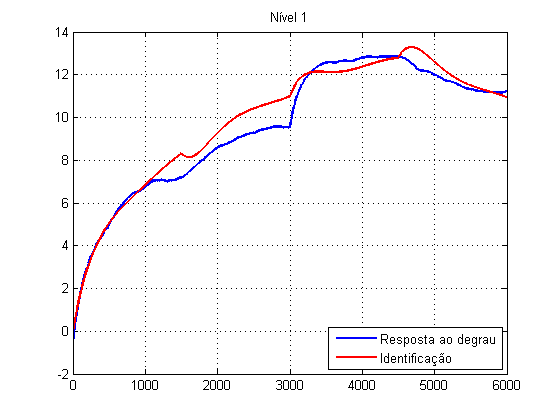
\includegraphics[height=0.15\paperheight,keepaspectratio]{img/ident2_h1.png} &
		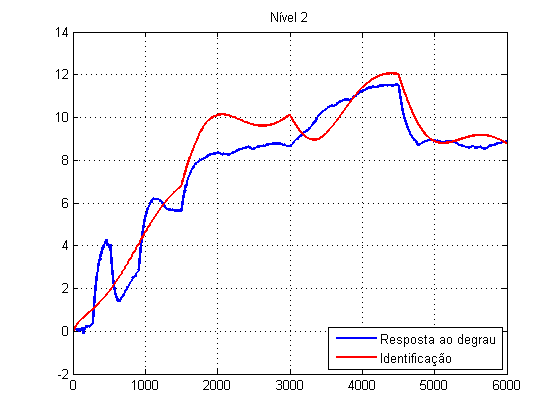
\includegraphics[height=0.15\paperheight,keepaspectratio]{img/ident2_h2.png} \\
		(a) Nível 1 &
		(b) Nível 2 \\
		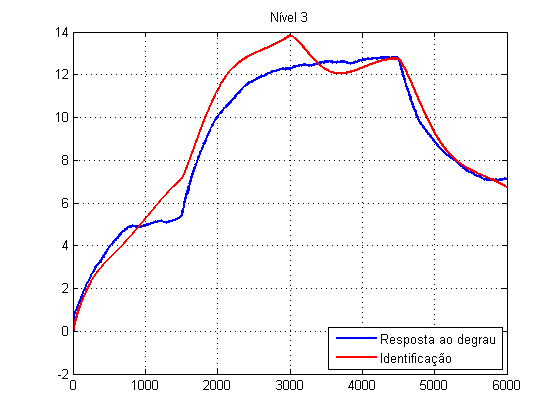
\includegraphics[height=0.15\paperheight,keepaspectratio]{img/ident2_h3.png} &
		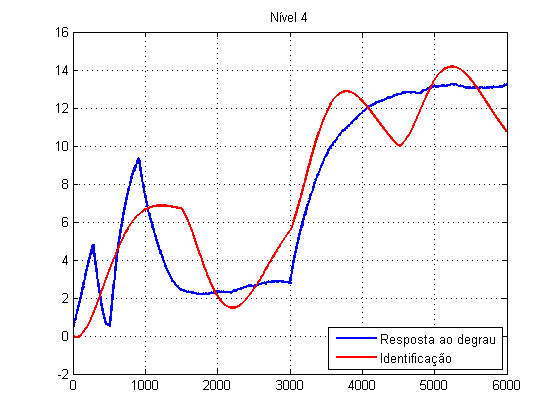
\includegraphics[height=0.15\paperheight,keepaspectratio]{img/ident2_h4.png} \\
		(c) Nível 3 &
		(d) Nível 4
	\end{tabular}
	\caption{\label{imgID_45Results} Identificação 2 - 6000 segundos}
\end{figure}

\begin{align*}
	& A_2 =
	\begin{bmatrix}
		     0.999 &    0.0002 &   0.000456 &  3.182e-05 \\
		-0.0001421 &         1 & -0.0001671 &  0.0002886 \\
		-0.0005784 & 0.0003516 &     0.9999 &  0.0001039 \\
		 0.0006769 & -0.001255 &  0.0006098 &     0.9999
	\end{bmatrix}\\
	& B_2 =
	\begin{bmatrix}
		-0.0004175 &  0.0005107 \\
		 0.0006248 & -0.0005959 \\
		 0.0002711 & -0.0002032 \\
		-0.0002449 &  0.0002294
	\end{bmatrix}
\end{align*}

\newpage \item Identificação III:
\begin{figure}[H]
	\centering
	\begin{tabular}{cc}
		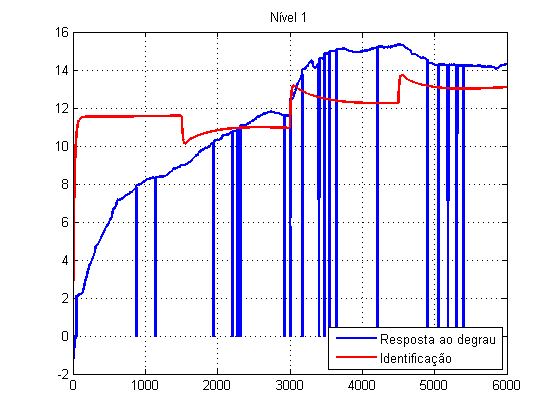
\includegraphics[height=0.15\paperheight,keepaspectratio]{img/ident3_h1.png} &
		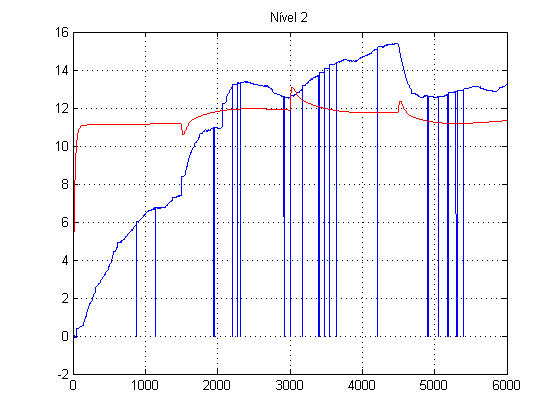
\includegraphics[height=0.15\paperheight,keepaspectratio]{img/ident3_h2.png} \\
		(a) Nível 1 &
		(b) Nível 2 \\
		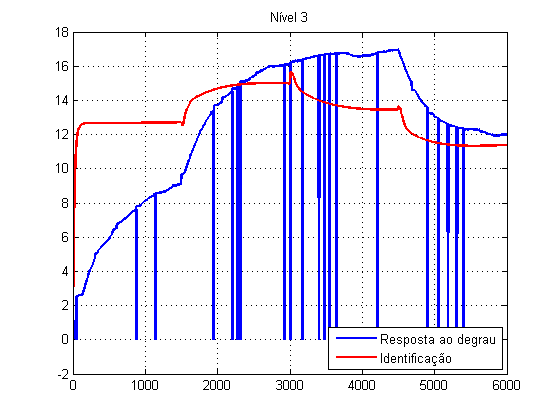
\includegraphics[height=0.15\paperheight,keepaspectratio]{img/ident3_h3.png} &
		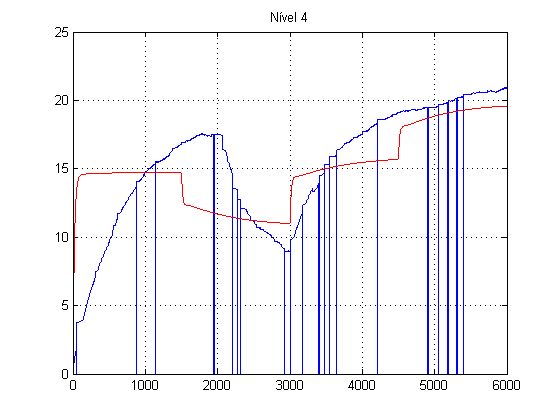
\includegraphics[height=0.15\paperheight,keepaspectratio]{img/ident3_h4.png} \\
		(c) Nível 3 &
		(d) Nível 4
	\end{tabular}
	\caption{\label{imgID_6Results} Identificação 3 - 6000 segundos}
\end{figure}

\begin{align*}
	& A_3 =
	\begin{bmatrix}
		   0.9834 & 0.02014 & -0.007577 &  -0.00362 \\
		  -0.0117 &   1.019 & -0.009873 & -0.003866 \\
		-0.009733 & 0.02102 &    0.9863 & -0.004788 \\
		 -0.02114 & 0.02447 & -0.008362 &    0.9952
	\end{bmatrix} \\
	& B_3 =
	\begin{bmatrix}
		-0.007073  & 0.009851 \\
		-0.004253  & 0.006861 \\
		-0.002624  & 0.005544 \\
		-0.009936  &  0.01346
	\end{bmatrix}
\end{align*}
\end{itemize}

Observou-se ao se aplicar os métodos de obtenção de ganhos pro controlador, descritos nos capítulos anteriores, se obtém valores muito altos ou excessivamente baixos, o que torna o controle inviável do ponto de vista prático devido a saturação dos atuadores que não foram levados em conta no projeto.

\subsection{Identificação Caixa-Cinza}

Nesta abordagem obtêm-se os parâmetros aferindo diretamente do sistema ou por meio de respostas à entradas controladas e utiliza-se as \jhhref{eqModLinear}{equações} para definir o modelo linear identificado. A \jhhref{tabDescPlanta}{Tabela} apresenta os valores das dimensões mensuráveis do tanque e da aceleração da gravidade. Os demais parâmetros serão identificados em 4 pontos, escolhidos por observação, que comporão as regras do modelo TS. 

Escolheu-se realizar-se a identificação para o funcionamento das bombas a 42\% e 45\% de suas capacidades. Nota-se que abaixo de 30\% não há resposta aparente e durante todo este trabalho limitou-se a atuar abaixo de 70\% de sua potência máxima, uma vez que este valor foi observado como limiar seguro de utilização. Os valores de $\gamma$ são obtidos enviando tensões constantes para cada bomba e verificando a proporção de fluído enviado para os tanques respectivos. Como o comportamento real da bomba é não linear, esses valores são identificados para cada uma das regras.

De forma semelhante, as constantes de fluxo $k$ são identificadas aferindo-se o volume enviado aos tanques, para uma dada tensão constante num tempo fixo. A taxa volume/tempo é utilizada como fluxo médio, $k_i$ é obtido dividindo o fluxo médio $i$ pela tensão $i$ utilizada. Optou-se por realizar a identificação do sistema em uma configuração em fase mínima, visando a simplificação dos cálculos e ilustração das práticas abordadas.

\begin{table}[!ht]
	\caption{Tensões Escolhidas}
	\label{tabIdentKs}
	\small
	\centering
	\scalebox{1}{
		\begin{tabular}{|c|c|c|c|c|c|c|}
			\hline
			Identificação & Tensão ($v_i$)&  $\gamma_1$ & $\gamma_2$ & Ganho 1 ($k_1$) & Ganho 2 ($k_2$) \\ \hline
			1 & 42\% & 0.8980 & 0.6810 & 7.4044 $cm^3/Vs$ & 7.1022 $cm^3/Vs$\\ \hline
			2 & 45\% & 0.8276 & 0.6827 & 8.1801 $cm^3/Vs$ & 7.3339 $cm^3/Vs$\\ \hline
		\end{tabular}
	}
\end{table}
Realiza-se então a identificação do modelo, a partir dos estados estacionários, nos 4 pontos dados pela interpolação destes conjuntos. Os resultados obtidos são exibidos a seguir:

\begin{table}[!ht]
	\caption{Pontos de Operação da Planta Instalada}
	\label{tabPontOp}
	\small
	\centering
	\scalebox{1}{
		\begin{tabular}{|c|c|c|c|c|c|c|}
			\hline
			Sistema & Bomba 1 ($\bar{v_1}$) & Bomba 2 ($\bar{v_1}$) & Nível 1 ($\bar{h_1}$) & Nível 2 ($\bar{h_2}$) & Nível 3 ($\bar{h_3}$) & Nível 4 ($\bar{h_4}$) \\ \hline
			1 & 42\% & 42\% & 11.1024 cm &  9.4410 cm &  8.7849 cm & 17.4466 cm \\ \hline
			2 & 42\% & 45\% & 16.3767 cm &  16.1350 cm & 11.4907 cm & 20.5671 cm \\ \hline
			3 & 45\% & 42\% & 15.0037 cm &  13.9138 cm & 20.7899 cm & 19.5759 cm \\ \hline
			4 & 45\% & 45\% & 18.0278 cm &  18.8761 cm & 18.3048 cm & 19.6136 cm \\	\hline
		\end{tabular}
	}
\end{table}

Obtém-se então um modelo como o proposto na  \jhhref{eqModTakSug}{Equação} composto por 4 regras. As matrizes que compõem cada regra são apresentadas a seguir:

\begin{align*} % Planta 1
	& A_1 =
	\begin{bmatrix}
	-0.0177 &     0   &  0.0057   &      0 \\
         0  & -0.0131 &       0   &  0.0010 \\
         0  &       0 &  -0.0057  &      0 \\
         0  &       0 &        0  & -0.0010 
	\end{bmatrix}
	& B_1 =
	\begin{bmatrix}
    0.1397  &      0 \\
		0   & 0.1016 \\
		0   & 0.0476 \\
	0.0159  &      0
	\end{bmatrix}
\end{align*}

\begin{align*} % Planta 2
	& A_2 =
	\begin{bmatrix}
		-0.0123 &       0 &    0.0048 &        0 \\
			0  & -0.0084 &         0 &   0.0008 \\
			0  &       0 &   -0.0048 &        0 \\
			0  &       0 &         0 &  -0.0008
	\end{bmatrix}
	& B_2 =
	\begin{bmatrix}
		0.1397 &        0 \\
			0  &  0.1052 \\
			0  &  0.0489 \\
		0.0159 &        0
	\end{bmatrix}
\end{align*}

\begin{align*} % Planta 3
	& A_3 =
	\begin{bmatrix}
	   -0.0140 &       0 &   0.0024 &        0 \\
			0  & -0.0101  &       0  &  0.0017 \\
			0  &       0  & -0.0024  &       0 \\
			0  &       0  &       0  & -0.0017
	\end{bmatrix}
	& B_3 =
	\begin{bmatrix}
	    0.1422 &       0 \\
			0  &  0.1016 \\
			0  &  0.0476 \\
		0.0296 &       0 
	\end{bmatrix}
\end{align*}
		
\begin{align*} % Planta 4
	& A_4 =
	\begin{bmatrix}
   -0.0119 &       0  &  0.0030 &        0 \\
		0  & -0.0080  &       0 &   0.0017 \\
		0  &       0  & -0.0030 &        0 \\
		0  &       0  &       0 &  -0.0017
	\end{bmatrix}
	& B_4 =
	\begin{bmatrix}
	0.1422 &       0 \\
		0  &  0.1052 \\
		0  &  0.0489 \\
	0.0296 &       0
	\end{bmatrix}
\end{align*}

Aplicando-se então o  \jhhref{teoControlador}{Teorema} obtém-se os ganhos a seguir:
\begin{table}[!ht]
	\caption{Ganhos aplicados à planta}
	\label{tabGanhosReais}
	\small
	\centering
	\scalebox{1}{
	\begin{tabular}{|c|c|}
		\hline
		Regra & Ganho \\ \hline
		1 & $ K = 
		\begin{bmatrix}
			-10.1267 &  -0.1726 & -0.0693 &  -0.0304 & 7.4632  &  0.0782 \\
			0.4704   & -8.9962  &  0.0234 &  -0.0081 & -0.1735 & 11.3821
		\end{bmatrix}$ \\[10pt] \hline
		2 & $ K = 
		\begin{bmatrix}
			-10.1655 &  -0.1445 &  -0.0628 &  -0.0301 &  7.4634 & 0.0680 \\
			0.3944   & -8.7470  &  0.0221  & -0.0071  & -0.1460 & 11.0130
		\end{bmatrix}$ \\[10pt] \hline
		3 & $ K = 
		\begin{bmatrix}
			-9.7178 &  -0.2288 &  -0.0433 &  -0.0878 &   7.1828 &   0.0979 \\
			0.5970  & -8.9866  & -0.0014  & -0.0096  & -0.2192  & 11.3719
		\end{bmatrix}$ \\[10pt] \hline
		4 & $ K = 
		\begin{bmatrix}
			-9.7327 &  -0.2180 &  -0.0472 &  -0.0874 &   7.1831 &   0.0939 \\
			0.5519  & -8.7291  &  0.0082  & -0.0090  & -0.2028  & 11.0068
		\end{bmatrix}$ \\[10pt] \hline
	\end{tabular}
	}
\end{table}

\section{CLP}
Os ganhos obtidos a partir da identificação do modelo foram implementados no CLP utilizando um diagrama de bloco de funções e uma rotina em texto estruturado. A \jhhref{figCLPCLPbf}{Figura} a seguir apresenta o programa principal. 

\begin{figure}[H]
	\centering
	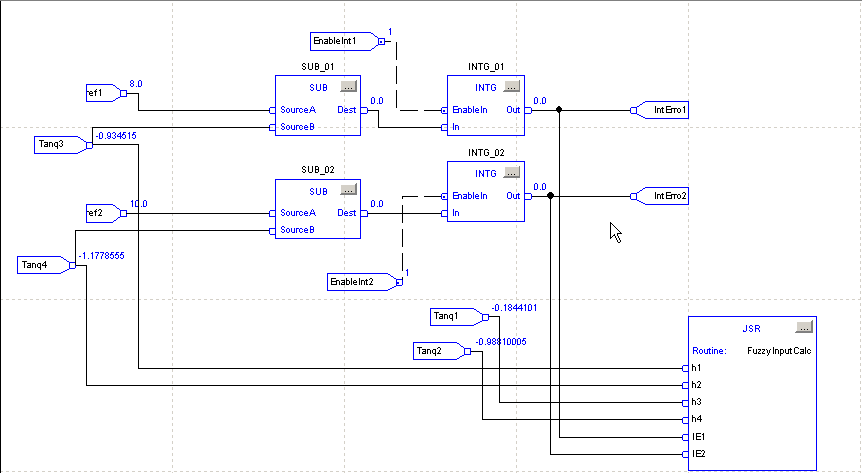
\includegraphics[width=\textwidth]{img/clp_bf2.png}
	\caption{Programa Principal}
	\label{figCLPCLPbf}
\end{figure}

O controlador recebe os estados atuais do sistema e os erros acumulados das variáveis controladas. A rotina textit{FuzzyInputCalc} implementa o controlador fuzzy a partir destas entradas e dos ganhos já apresentados assinalando às variáveis de saída o valor da tensão nas bombas desejado. A \jhhref{figCLPTags1}{Figura} a seguir apresenta as variáveis definidas no trabalho. O código em texto estruturado do bloco FuzzyInputCalc acima pode ser visto no Anexo A2.

\begin{figure}[H]
	\centering
	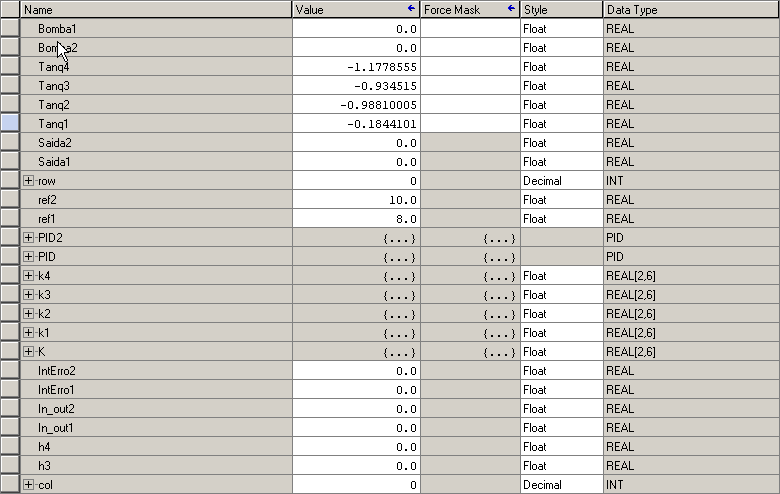
\includegraphics[width=0.7\textwidth]{img/tags1.png}\\
	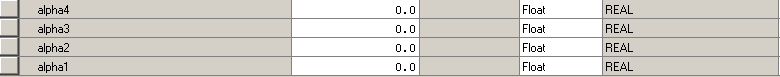
\includegraphics[width=0.7\textwidth]{img/tags2.png}
	\caption{Variáveis do programa}
	\label{figCLPTags1}
\end{figure}

Os resultados obtidos são apresentados na \jhhref{secResImp}{seção} a seguir.

\selectlanguage{brazil}%

